%%%%%%%%%%%%%%%%%%%%%%%%%%%%%%%%%%%%%%%%%%%%%%%%%
% openshift.tex
% 
% Latex source to be converted to HTML by tex4ht
%
%%%%%%%%%%%%%%%%%%%%%%%%%%%%%%%%%%%%%%%%%%%%%%%%%
\documentclass{article}

%%%%%%%%%%%%%%%%%%%%%%%%%%%%%%%%%%%%%%%%%%%%%%%%%
% PREAMBLE
%%%%%%%%%%%%%%%%%%%%%%%%%%%%%%%%%%%%%%%%%%%%%%%%%
% Import common configurations and custom functions
%%%%%%%%%%%%%%%%%%%%%%%%%%%%%%%%%%%%%%%%%%%%%%%%%
% PREAMBLE
%%%%%%%%%%%%%%%%%%%%%%%%%%%%%%%%%%%%%%%%%%%%%%%%%
\usepackage{hyperref}
\usepackage{listings}
\usepackage{color}
\usepackage[dvipsnames]{xcolor}
\usepackage{float}
\usepackage{graphicx}
\usepackage{tikz,tikz-dependency}
\usepackage{ifthen}
\usetikzlibrary{calc}
\usetikzlibrary{automata,positioning,external,shapes,arrows,chains,matrix,scopes,backgrounds}
\usepackage{enumerate}
% The following is for tikz externalization configuration which allows
% tikZ diagrams to render correctly while being processed by htlatex 
% http://tex.stackexchange.com/questions/158551/using-htlatex-with-tikz-dependency#158921
%%%%%%%%%%%%%%%%%%%%%%%%%%%%%%%%%%%%%%%%%%%%%%%%%
\tikzset{
    tex4ht inc/.style={
        /pgf/images/include external/.code={%
            \includegraphics[]{##1.svg}%
        }

    }
}
\tikzset{
 external/system call/.add={}
      ; inkscape -z -f "\image.pdf" -l "\image.svg"
}
\makeatletter
\@ifpackageloaded{tex4ht}{
    \tikzexternalize[mode=only graphics]
}{
    \tikzexternalize
}
\makeatother

% Removes section numbers
\makeatletter
\renewcommand\thesection{}
%\renewcommand\thesubsection{\@arabic\c@section.\@arabic\c@subsection}
\renewcommand\thesubsection{}
\makeatother

%%%%%%%%%%%%%%%%%%%%%%%%%%%%%%%%%%%%%%%%%%%%%%%%%
% COLOR DEFINITIONS
%%%%%%%%%%%%%%%%%%%%%%%%%%%%%%%%%%%%%%%%%%%%%%%%%
\tikzstyle{red}     = [fill=red!30!white]
\tikzstyle{orange}  = [fill=orange!30!white]
\tikzstyle{yellow}  = [fill=yellow!30!white]
\tikzstyle{green}   = [fill=green!30!white]
\tikzstyle{blue}    = [fill=blue!30!white]
\tikzstyle{teal}    = [fill=teal!30!white]
\tikzstyle{purple}  = [fill=purple!30!white]
\tikzstyle{magenta} = [fill=magenta!30!white]
\tikzstyle{gray}    = [fill=gray!30!white]
%\tikzstyle{black}   = [fill=black!30!white]

%%%%%%%%%%%%%%%%%%%%%%%%%%%%%%%%%%%%%%%%%%%%%%%%%
% DEFINE STACK COLORS
%%%%%%%%%%%%%%%%%%%%%%%%%%%%%%%%%%%%%%%%%%%%%%%%%
\definecolor{DEFINE_USR_COLOR}{HTML}{006699}
\definecolor{DEFINE_KRN_COLOR}{HTML}{003366}
\definecolor{DEFINE_HW_COLOR}{HTML}{000033}
\definecolor{DEFINE_CET_COLOR}{HTML}{339999}
\definecolor{DEFINE_CE_ARQ_COLOR}{HTML}{003333}

\tikzstyle{DK_COLOR}  = [fill=blue!30!white]
\tikzstyle{ARQ_COLOR} = [fill=gray!30!white]
\tikzstyle{OS_COLOR}  = [fill=black!50!white]
\tikzstyle{USR_COLOR} = [fill=DEFINE_USR_COLOR]
\tikzstyle{KRN_COLOR} = [fill=DEFINE_KRN_COLOR]
\tikzstyle{HW_COLOR}  = [fill=DEFINE_HW_COLOR]
\tikzstyle{CET_COLOR} = [fill=DEFINE_CET_COLOR]
\tikzstyle{CE_ARQ_COLOR} = [fill=DEFINE_CE_ARQ_COLOR]
\tikzstyle{HM_COLOR}  = [fill=cyan!30!white]
%%%%%%%%%%%%%%%%%%%%%%%%%%%%%%%%%%%%%%%%%%%%%%%%%
% STACK DIAGRAM DEFINITIONS
%%%%%%%%%%%%%%%%%%%%%%%%%%%%%%%%%%%%%%%%%%%%%%%%%
\tikzstyle{layer}      = [rectangle, thick, rounded corners]
\tikzstyle{core_stack} = [layer, minimum width=11cm,minimum height=1cm, text = white]
\tikzstyle{user_stack} = [layer, minimum width=4cm,minimum height=1cm]
\tikzstyle{app_stack}  = [layer, minimum width=4.5cm,minimum height=3cm]
\tikzstyle{container}  = [layer, purple,minimum width=0.5cm,minimum height=0.5cm]

\tikzstyle{OS_LAYER}  = [app_stack]
\tikzstyle{ARQ_LAYER} = [app_stacK]
\tikzstyle{CET_LAYER} = [user_stack, CET_COLOR]
\tikzstyle{USR_LAYER} = [core_stack, USR_COLOR, minimum height=4.5cm, label={[label distance=-0.75cm]270:\color{white}Userspace}]
\tikzstyle{KRN_LAYER} = [core_stack, KRN_COLOR, below= 0cm of USR]
\tikzstyle{HW_LAYER}  = [core_stack, HW_COLOR, below of=KRN]
\tikzstyle{DK_LAYER}  = [user_stack, DK_COLOR]
\tikzstyle{HM_LAYER}  = [user_stack, HM_COLOR]

%%% NEW DEFS
\tikzstyle{OS_LAYER2} = [app_stack, OS_COLOR,fill=black!50!white, label={[label distance=-0.75cm]270:OpenShift}]

\tikzstyle{c_temp} = [layer,minimum width=0.5cm,minimum height=0.5cm]
\tikzstyle{c_empt} = [c_temp]
\tikzstyle{c_move} = [c_temp, draw, dotted]
\tikzstyle{c_full} = [c_temp, purple, draw=black, thin]
\tikzstyle{mw}     = [minimum width=5.0cm]

\tikzstyle{c}    = [container, draw=black, thin]
\tikzstyle{pod}  = [thick, opacity=0.5, rounded corners]
\tikzstyle{NS}   = [thick, draw, dotted] %Namespace
\tikzstyle{blank}= [c_temp, OS_COLOR, thick, c_move]
\tikzstyle{pod}  = [thick, opacity=0.4, rounded corners, circle]
\tikzstyle{box} = [rectangle, thick, rounded corners, text= white]
\tikzstyle{link} = [-, thick, opacity=0.3]

\definecolor{keyword}{rgb}{0,0,0}
\definecolor{comment}{rgb}{0,0,0}
\definecolor{string}{rgb}{0,0,0}

% lstlisting configs for code syntax formatting
\lstdefinestyle{Java} {
  frame=tb,
  language=Java,
  aboveskip=3mm,
  belowskip=3mm,
  showstringspaces=false,
  columns=flexible,
  basicstyle={\large\ttfamily},
  numbers=none,
  numberstyle=\textcolor{gray},
  keywordstyle=\textcolor{red!75},
  commentstyle=\textcolor{dkgreen},
  stringstyle=\textcolor{blue},
  moredelim=[is][\textcolor{black!75}]{|}{|},
  breaklines=false,
  breakatwhitespace=true,
  tabsize=3,
  belowskip=-0.5em %\baselineskip
}

\lstdefinestyle{shell} {
  basicstyle=\ttfamily,
  showstringspaces=false,
  keywordstyle=\textcolor{keyword},
  commentstyle=\textcolor{comment},
  stringstyle=\textcolor{string},
  belowskip=-\baselineskip
  %belowskip=-\baselineskip
}

%%%%%%%%%%%%%%%%%%%%%%%%%%%%%%%%%%%%%%%%%%%%%%%%
% Tikz Functions
%%%%%%%%%%%%%%%%%%%%%%%%%%%%%%%%%%%%%%%%%%%%%%%%
\newcommand{\containers}[4] {
  \xdef\cmax{7}
  \def\id{#1}                   % #1 = id 
  \pgfmathsetmacro\nc{int(#2)}  % #2 = number of containers
  \pgfmathsetmacro\nfc{int(#3)} % #3 = number of full containers 
  \tikzstyle{LOCATION} = {#4}   % #4 = location
  \node[#4] (loc) {}; 

  \node[LOCATION] (loc) {};
  % Initialize container nodes
  \foreach \x in {0,...,7}{
    \node[] (C\x_\id) {};
  }

  \xdef\sp{loc};     % starting position
  \xdef\ct{c_full}; % container type
  \foreach \x in {0,...,\cmax} {
    {\ifthenelse{\x < \nc}
      { {\ifthenelse{\x < \nfc }
          {\xdef\ct{c_full};}
          {\xdef\ct{c_move};}
        }
      }
      { \xdef\ct{c_empt};}
    }
    \node[\ct, right=of \sp] (C\x_\id) {};
    \xdef\sp{C\x_\id};
  };

  %{\ifthenelse{\nc < 4}{}{
  %Container label with spanning arrows
  \node[fit=(C0_\id)(C1_\id)(C2_\id)(C3_\id)(C4_\id)(C5_\id)(C5_\id)(C6_\id)(C7_\id)] (all) {};
  \node[above= -0.15cm of all.north ] (C_LABEL_\id) {\small Containers};
  \path[->, to path={-| (\tikztotarget)}]
  (C_LABEL_\id.west) edge (C0_\id.north)
  (C_LABEL_\id.east) edge (C7_\id.north);
  
}

\newcommand{\moby}[4] {
  \xdef\cmax{7}
  \def\id{#1}                   % #1 = id 
  \pgfmathsetmacro\nc{int(#2)}  % #2 = number of containers
  \pgfmathsetmacro\nfc{int(#3)} % #3 = number of full containers 
                                % #4 = location
  % Initialize container nodes
  \foreach \x in {0,...,7}{
    \node[] (C\x_\id) {};
  }
  % Instantiate moby and container nodes
  \node[DK_LAYER, DK_COLOR, #4] (DK_\id) {Moby};
  \node[above left= 0.1cm and 0cm of DK_\id.north west] (sp) {};

  \xdef\sp{sp};     % starting position
  \xdef\ct{c_full}; % container type
  \foreach \x in {0,...,\cmax} {
    {\ifthenelse{\x < \nc}
      { {\ifthenelse{\x < \nfc }
          {\xdef\ct{c_full};}
          {\xdef\ct{c_move};}
        }
      }
      { \xdef\ct{c_empt};}
    }
    \node[\ct, right=of \sp] (C\x_\id) {};
    \xdef\sp{C\x_\id};
  };

  {\ifthenelse{\nc < 4}{}{
  %Container label with spanning arrows 
  \node[above= 0.5cm of DK_\id.north ] (C_LABEL_\id) {Containers};
  \path[->, to path={-| (\tikztotarget)}]
  (C_LABEL_\id.west) edge (C0_\id.north)
  (C_LABEL_\id.east) edge (C7_\id.north);
  }};
}
\newcommand{\host}[4]{
  \def\id{#1}  % #1 = id
  \def\nc{#2}  % #2 = number of containers
  \def\nfc{#3} % #3 = number of full containers
               % #4 = location
  % Initialize nodes
  \foreach \x in {0,...,7}
    \node[] (C\x_\id) {};
    \node[] (DK_\id) {};
    \node[] (OS_\id) {};

  \node[OS_LAYER,fit=(DK_\id)] at (#4) (OS_\id) {};
  \moby{#1}{#2}{#3}{above = 0cm of OS_\id.center, anchor=center};
  \node[HM_LAYER, mw, below= 0cm of OS_\id.south, anchor=north] (HM_\id) {Host Machine \id};
}

\newcommand{\OpenShift}[4]{
  \def\id{#1}  % #1 = id
  \def\nc{#2}  % #2 = number of containers
  \def\nfc{#3} % #3 = number of full containers
               % #4 = location
  % Initialize nodes
  \foreach \x in {0,...,7}
    \node[] (C\x_\id) {};
    \node[] (DK_\id) {};
    \node[] (OS_\id) {};

  \node[OS_LAYER,fit=(DK_\id), #4] (OS_\id) {};
  \moby{#1}{#2}{#3}{above = 0cm of OS_\id.center, anchor=center};
}

\newcommand{\Arquillian}[2]{
  \def\id{#1}  % #1 = id
               % #2 = location

  \node[] (CET_\id) {};
  \node[ARQ_LAYER, fit=(CET_\id), #2] (ARQ_\id) {};
  \node[CET_LAYER, above = 0cm of ARQ_\id.center, anchor=center] (CET_\id) {CE-Testsuite};
}

\newcommand{\pods}[5]{
  \xdef\id{#1}
  \pgfmathtruncatemacro{\numPods}{#2-1}
  \xdef\numCons{#3-1};
  \pgfmathtruncatemacro{\cpp}{2 - 1} %containers per pod
  \xdef\cfit{} % containers for pod to fit
  \xdef\pfit{} % pods for namespace to fit

  \node[#4] (BASE) {};
  \xdef\lcp{BASE}; % last container position
  \xdef\sbc{}; % space between container
  \pgfmathsetmacro\r{#3}
 % Initialize pods
  \foreach \x in {0,...,\numPods}{
    \pgfmathsetmacro\pods{int(#2 - \x)}
    {\ifthenelse{\r > \pods }
    { % if 
      \xdef\numCons{1}
      \pgfmathsetmacro\r{int(\r - 2)}
      \xdef\r{\r}
    }
    { % else
      \xdef\numCons{0};
      \pgfmathsetmacro\r{int(\r - 1)}
      \xdef\r{\r}
    }
    };
    %\node[] at (-5,\x) {\r \pods \numCons};

    \foreach \y in {0,...,\numCons}{
      \node[c_full, right= \sbc of \lcp] (P\x_C\y_#1) {};
      \xdef\lcp{P\x_C\y_#1}
      \xdef\cfit{\cfit(P\x_C\y_#1)} % add container to be fitted
      \xdef\sbc{}; %space between containers
    }

    % randomly generate color for pod
    \pgfmathparse{rnd}
    \pgfmathtruncatemacro{\cc}{(\id)*0.4}
    \xdefinecolor{rColor}{rgb}{\cc, 0.7, \pgfmathresult}

    \node[pod, fill=rColor, fit=\cfit] (P\x_\id) {};
    %\pgfmathparse{rnd * \x}

    \xdef\cfit{};
    \xdef\sbc{0cm and 0.5cm}; %space between containers
    \xdef\pfit{\pfit(P\x_\id)} % add container to be fitted
    }
    #5
}

\newcommand{\namespace}[4]{
  \pods{#1}{#2}{#3}{#4}{\node[fit=\pfit] (NS_#1) {};};
  \node[NS, fit=\pfit] (NS_#1) {};
  \node[above=0cm of NS_#1.north] (NS_#1_LABEL) {Namespace #1};
  %\node[NS, fill=gray!10, fit=\pfit] (NS_#1) {};
  \pods{#1}{#2}{#3}{#4}{};
  %\pods{#1}{#2}{#3}{#4}{};
}

\newcommand{\cube}[4] {
  \def\id{#1}
  \def\size{#2}
  \def\color{#3}
  \tikzstyle{location} = [#4]

  \def\x{\size * 0.4}
  \def\y{\size * 0.5}
  \def\z{\size * 1.0}

  \tikzstyle{coor} = [shape=coordinate]
  \node[circle, location] (\id) {};

  \node[coor, below left =\x cm and \y cm of \id] (S_\id) {S};
  \node[coor, above=\z cm and 0cm of S_\id] (A_\id) {A};
  \node[coor, above right=\y cm and \x cm of A_\id] (B_\id) {B};
  \node[coor, above right=\y cm and \x cm of S_\id] (C_\id) {C};
  \node[coor, right=0.0cm and \z cm of S_\id] (D_\id) {D};
  \node[coor, above=\z cm and 0.0cm of D_\id] (E_\id) {E};
  \node[coor, above right=\y cm and \x cm of E_\id] (F_\id) {F};
  \node[coor, above right=\y cm and \x cm of D_\id] (G_\id) {G};

  \tikzstyle{face} = [black]

  \draw[face, fill=\color!30] (S_\id) -- (C_\id) -- (G_\id) -- (D_\id) -- cycle; % Bottom Face
  \draw[face, fill=\color!30] (S_\id) -- (A_\id) -- (E_\id) -- (D_\id) -- cycle; % Back Face
  \draw[face, fill=\color!10] (S_\id) -- (A_\id) -- (B_\id) -- (C_\id) -- cycle; % Left Face
  \draw[face, fill=\color!20,opacity=0.8] (D_\id) -- (E_\id) -- (F_\id) -- (G_\id) -- cycle; % Right Face
  \draw[face, fill=\color!20,opacity=0.6] (C_\id) -- (B_\id) -- (F_\id) -- (G_\id) -- cycle; % Front Face
  \draw[face, fill=\color!20,opacity=0.8] (A_\id) -- (B_\id) -- (F_\id) -- (E_\id) -- cycle; % Top Face

  \node[coor] (\id_center) at ($(S_\id)!0.5!(F_\id)$)  {};
  \node[coor] (\id_north)  at ($(A_\id)!0.5!(F_\id)$)  {};
  \node[coor] (\id_east)   at ($(D_\id)!0.5!(F_\id)$)  {};
  \node[coor] (\id_south)  at ($(S_\id)!0.5!(G_\id)$)  {};
  \node[coor] (\id_west)   at ($(S_\id)!0.5!(B_\id)$)  {};

  %\node[fit=(S_\id)(F_\id)] (\id) {};
  %\tikzstyle{cube}= [fit=(S_\id)(A_\id)(B_\id)(C_\id)(D_\id)(E_\id)(F_\id)(G_\id)];
  %\node[circle, draw, location] (test\id) {};
}

% Registry \regID is labeled in the format R<Registry number> 
% (e.g. R0 would represent Registry 0) while the cubes are 
% separated into labels of R\idC\row\col 
% (e.g. R0C00 Cube row 0 and col 0 of Registry 0)
\newcommand{\registry}[5] {
  \def\regID{#1}
  \pgfmathsetmacro{\cubesize}{#2};
  \pgfmathsetmacro{\rows}{int(#3 - 1)}
  \pgfmathsetmacro{\cols}{int(#4 - 1)}
  \tikzstyle{loc} = [#5]

  \node[loc] (LOCATION) {};

  \foreach \r in {0,...,\rows}{
    \foreach \c in {0,...,\cols}{
      \pgfmathsetmacro{\vdis}{\r * \cubesize}
      \pgfmathsetmacro{\hdis}{\c * \cubesize}
      %\pgfmathsetmacro{\num}{int(\c + (\r * #4))}
      %\node[above right= \vdis cm and \hdis cm of LOCATION] (Cuve\num R) {};
      \cube{\regID C\r \c}{\cubesize}{gray}{above right= \vdis cm and \hdis cm of LOCATION};
    }
  }

  \node[fit=(S_\regID C00) (F_\regID C\rows \cols)] (\regID) {};
  \node[above= -0.10cm of \regID] (\regID_label) {\small Registry};
}

%\newcommand{\template}[4] {
%  \def\tempID{#1}
%  \pgfmathsetmacro{\size}{#2}
%  \pgfmathsetmacro{\minWidth}{\size * 0.75}
%  \def\color{#3}
%  \tikzstyle{tempID_location} = [#4]
%
%  \tikzstyle{template} = [rectangle, draw,fill = \color, minimum height = \size cm, 
%                          minimum width = \minWidth cm]
%  \node[template, tempID_location] (\tempID) {};
%}
%
% CAT0T00 = Catalog 0, template on row 0 column 0
%

\newcommand{\pod}[5]{
  \def\podID{#1}
  \pgfmathsetmacro{\conSize}{#2}
  \pgfmathsetmacro{\rows}{int(#3 - 1)}
  \pgfmathsetmacro{\cols}{int(#4 - 1)}
  \tikzstyle{loc} = [#5]
  \node[loc] (\podID_location) {};

  \foreach \r in {0,...,\rows}{
    \foreach \c in {0,...,\cols}{
      \pgfmathsetmacro{\vdis}{(\r * \conSize)}
      \pgfmathsetmacro{\hdis}{(\c * \conSize)}
      \node[c_full, above right= \vdis cm and \hdis cm of \podID_location] (\podID C\r \c) {};
    }
  }

  % randomly generate color for pod
  \pgfmathparse{rnd}
  \pgfmathtruncatemacro{\cc}{(\rows + \cols)*0.4}
  \xdefinecolor{rColor}{rgb}{\cc, 0.7, \pgfmathresult}

  \node[pod, fill=rColor, fit=(\podID C00)(\podID C\rows \cols)] (\podID) {};
}

\newcommand{\project}[5] {
  \def\projectID{#1}
  \pgfmathsetmacro{\projectSize}{#2}
  \pgfmathsetmacro{\numCons}{(#3)}
  \pgfmathsetmacro{\numPods}{#4}
  \pgfmathsetmacro{\podRange}{int(\numPods - 1)}
   
  %\pgfmathsetmacro{\numCons}{(#3 - 1)}
  %\pgfmathsetmacro{\numPods}{(#4 - 1)}
  \tikzstyle{prevLoc} = [#5]
  \node[#5] (\projectID_location) {};  
  
  \pgfmathsetmacro{\consPerPod}{(\numCons / \numPods)}
  %\pgfmathsetmacro{\cl}{\nnumCons }
  %\foreach \np [count=\S from 1] in {0,...,\numPods}{
  \foreach \np in {0,...,\podRange}{
    \pgfmathsetmacro{\sep}{\np * ((\consPerPod+1)*\projectSize)}
    %\pgfmathsetmacro{\cons}{int((\numCons - (\consPerPod * \np)) / \numPods) + 1 }
    \pod{\projectID P\np}{\projectSize}{1}{\consPerPod}{right= 0cm and \sep cm of \projectID_location}
    %\node[right= 0cm and \sep cm of \projectID_location] (\projectID P\np) {\cl};
  }

  \node[NS, fit=(\projectID P0)(\projectID P\podRange)] (\projectID) {};
  %\node[above = 0cm of \projectID] (\projectID_label) {Project};
}

\newcommand{\router}[3]{
  \def\routerID{#1}
  \def\size{#2}
  \tikzstyle{loc} = [#3]
  
  \pgfmathsetmacro{\height}{\size * 0.25}
  \tikzstyle{router} = [rectangle, black, rounded corners, minimum height = \height cm, minimum width = \size cm]

  \node[router, fill=black!30, loc] (in_router) {};
  \node[thick, draw, rounded corners, black, fit=(in_router)] (\routerID) {};
  \node[router, fill=black!30, loc] (in_router2) {};

  \tikzstyle{light} = [circle, green, minimum width = 0.05ex]

  \node[light] (dot1) at (\routerID.center) {};
  \node[light, left = 0cm and 0cm of dot1] (dot2) {};
  \node[light, left = 0cm and 0cm of dot2] (dot3) {};

  \tikzstyle{antenna} = [draw,rectangle, rounded corners, fill=black!20, rotate=0, minimum height = 1cm]
  \node[antenna, above right= 0cm and 0.75cm of \routerID.north] (air) {};
  \node[above= 0cm of \routerID] () {Router};
  
}

% Make 3D template stack
\newcommand{\template}[4]{
  \def\tempID{#1}
  \pgfmathsetmacro{\size}{#2}
  \def\color{#3}
  \tikzstyle{location} = [#4]

  \def\x{\size * 0.4}
  \def\y{\size * 0.5}
  \def\z{\size * 1.0}

  \tikzstyle{coor} = [shape=coordinate]
  \node[circle, location] (\tempID) {};
 
  \node[coor, below left =\x cm and \y cm of \tempID] (A_\tempID) {A};
  \node[coor, right=0.0cm and \z cm of A_\tempID] (B_\tempID) {B};
  \node[coor, above right=\y cm and \x cm of A_\tempID] (C_\tempID) {C};
  \node[coor, above right=\y cm and \x cm of B_\tempID] (D_\tempID) {D};

  \tikzstyle{face} = [black, opacity=0.5]

  \draw[face, fill=\color!30] (A_\tempID) -- (C_\tempID) -- (D_\tempID) -- (B_\tempID) -- cycle; % Bottom Face

  \node[coor] (\tempID_center) at ($(A_\tempID)!0.5!(D_\tempID)$)  {};
  \node[coor] (\tempID_north) at ($(C_\tempID)!0.5!(D_\tempID)$)  {};
  \node[coor] (\tempID_east) at ($(B_\tempID)!0.5!(D_\tempID)$)  {};
  \node[coor] (\tempID_south) at ($(A_\tempID)!0.5!(B_\tempID)$)  {};
  \node[coor] (\tempID_west) at ($(A_\tempID)!0.5!(C_\tempID)$)  {};

  \node[fit=(A_\tempID)(D_\tempID)] (\tempID_fit) {};
  %\tikzstyle{cube}= [fit=(S_\id)(A_\id)(B_\id)(C_\id)(D_\id)(E_\id)(F_\id)(G_\id)];
  %\node[circle, draw, location] (test\id) {};
  
  % Writing
  %\node[above left =  0.2cm and 0.5cm of \tempID_center] (\tempID A1) {};
  %\node[above right = 0.2cm and 0.1cm of \tempID_center] (\tempID A2) {};
  %\draw  (\tempID A1) -- (\tempID A2);
  %\node[above left = 0.0cm and  0.7cm of \tempID_center] (\tempID B1) {};
  %\node[above right = 0.0cm and 0.3cm of \tempID_center] (\tempID B2) {};
  %\draw  (\tempID B1) -- (\tempID B2);
  %\node[below left = 0.0cm and  0.9cm of \tempID_center] (\tempID C1) {};
  %\node[below right = 0.0cm and 0.25cm of \tempID_center] (\tempID C2) {};
  %\draw  (\tempID C1) -- (\tempID C2);
  %\node[below left = 0.1cm and  0.9cm of \tempID_center] (\tempID D1) {};
  %\node[below right = 0.1cm and 0.2cm of \tempID_center] (\tempID D2) {};
  %\draw  (\tempID D1) -- (\tempID D2);
}

% Make 3D template stack
\newcommand{\catalog}[4] {
  \def\catID{#1}
  \pgfmathsetmacro{\tempSize}{#2}
  \pgfmathsetmacro{\tempNum}{int(#3 - 1)}
  \tikzstyle{loc} = [#4]
  \node[loc] (\catID_location) {};
    %\template{TTT}{1.2}{blue!50}{#4};

  \foreach \i in {0,...,\tempNum}{
    \pgfmathsetmacro{\vvdis}{\i * 0.25}
    \template{\catID T\i}{\tempSize}{blue}{above = \vvdis cm of \catID_location};
  }

  \node[fit=(\catID T0_fit)(\catID T\tempNum_fit)] (\catID) {};
  \node[above = -0.25cm of \catID] (\catID_label) {\small Catalog};
}

%\newcommand*{\var}[2]{%
%    \newcommand*{#1}{}% Error if already defined
%    \pgfmathsetmacro{#1}{#2}%
%}%
\newcommand{\openshift}[4] {
  \def\id{#1}
  \def\width{#2}
  \pgfmathsetmacro{\height}{#2 / 3}
  \tikzstyle{loc} = [#3]
  \node[#3] (LOCATION) {};
  \pgfmathsetmacro{\dis}{\height}
  
  \pgfmathsetmacro{\owidth}{\width / 3} 
  \pgfmathsetmacro{\oheight}{\height / 4}
   
  \tikzstyle{mw} = [minimum width=\width cm]
  \tikzstyle{mh} = [minimum height= \height cm]
  \tikzstyle{box} = [rectangle, thick, rounded corners, text= white]
  \tikzstyle{layer} = [box, mw, mh]
  
  \tikzstyle{OS_LAYER} = [box, OS_COLOR, minimum width = \owidth cm, minimum height = \oheight cm]

  \node[USR_COLOR, layer, label={[label distance=-0.55cm]270:\color{white}Userspace}, above = 0.45 cm  of LOCATION ] (\id_USR) {};
  \node[KRN_COLOR, layer, below = 0cm of \id_USR] (\id_KRN) {Kernel};
  \node[HW_COLOR,  layer, below = 0cm of \id_KRN] (\id_HW) {Hardware};
  
  \node[OS_LAYER, above=0.5cm of \id_USR.south] (\id_label) {\small OpenShift};
  
  \node [below = 0cm of \id_HW.south] (\id_HM) {Physical Machine};
  \path[->, thin, to path={-| (\tikztotarget)}]
    (\id_HM.west) edge (\id_HW.south west)
    (\id_HM.east) edge (\id_HW.south east);
  
  %\node [rotate=90, left = of \id_KRN.west, anchor=south] (\id_HM) {Host Machine};
  %    \path[->, thin, to path={|- (\tikztotarget)}]
  %    (\id_HM.east) edge (\id_USR.north west)
  %    (\id_HM.west) edge (\id_HW.south west);
      
  \node[fit=(\id_USR)(\id_KRN)(\id_HW)] (\id) {};
}









%%%%%%%%%%%%%%%%%%%%%%%%%%%%%%%%%%%%%%%%%%%%%%%%%
% DOCUMENT
%%%%%%%%%%%%%%%%%%%%%%%%%%%%%%%%%%%%%%%%%%%%%%%%%
\begin{document}

\centerline{\sc \large OpenShift}
\centerline{\sc Architecture for the Layperson }
\centerline{\url{https://github.com/openshift/origin}}

\vspace{1pc}

\section{Overview}
\hspace{3pc} Openshift is a \href{https://kyguy.github.io/src/containers/containers.html}{container} platform which facilitates the development and management of software applications across
distributed systems. Whether the components of these distributed systems be physical hosts, virtual machines or a combination of 
both, OpenShift reaps the benefits of available computing resources without the complexity typically tied with computing power. 

%\iffalse
%\fi
\begin{figure}
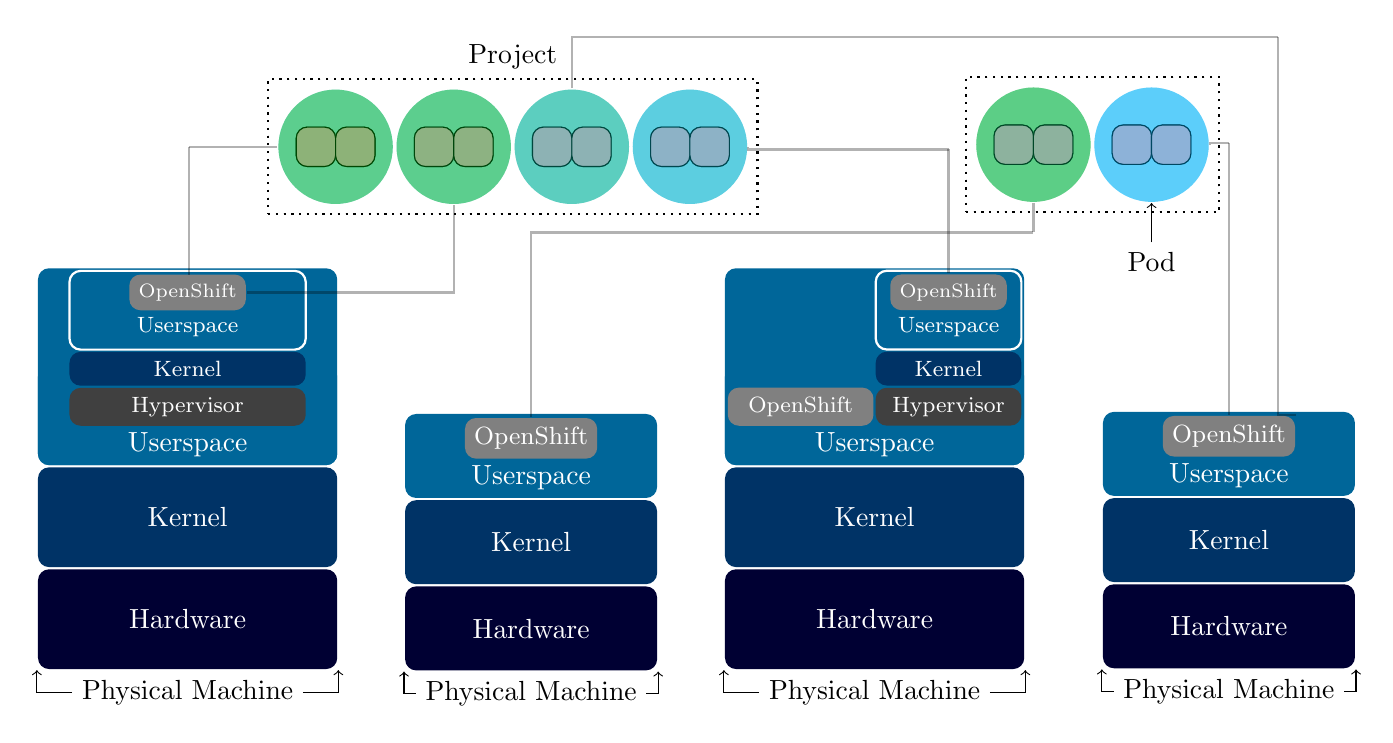
\begin{tikzpicture}[node distance = 1cm and 0cm]
  \tikzstyle{HYP_COLOR} = [fill=gray!50!black]
  
  % OpenShift layer
  \openshift{OS0}{3.2}{}{}
  %----------------------------------------------%
  % HOST 2
  \openshift{OS1}{3.8}{above left = -1.5cm and 2.5cm of OS0}{}
  \node[USR_COLOR, layer,minimum height = 2.5cm,
   label={[label distance=-0.55cm]270:\color{white}Userspace}, above = 0.45 cm  of LOCATION ] (OS1_USR) {};
  \tikzstyle{mw} = [minimum width= 3cm]
  \tikzstyle{mh} = [minimum width=0.25cm]
  \node[box, HYP_COLOR, mw, above=0.5cm of OS1_USR.south] (OS1_HYPER) {\footnotesize Hypervisor};
  \node[box, KRN_COLOR, mw, above= 0cm and 0cm of OS1_HYPER] (OS1_KRN) {\footnotesize Kernel};
  \node[box,USR_COLOR, draw=white, mw, minimum height = 1cm, above= 0cm and 0cm of OS1_KRN,
    label={[label distance=-0.55cm]270:\color{white}\footnotesize Userspace}] (OS1_USR2) {};
  \node[OS_LAYER, minimum width = 1.5 , above = 0.5cm and 0.0cm of OS1_USR2.south] (OS1_label2) {\scriptsize OpenShift};

  %----------------------------------------------%
  %\openshift{OS2}{3.2}{right = 0cm and 2cm of OS0}{} 
  %----------------------------------------------%

  % HOST 3
  \openshift{OS2}{3.8}{ above right = -1.5cm and 2.5cm of OS0}{}
  \node[USR_COLOR, layer,minimum height = 2.5cm,
   label={[label distance=-0.55cm]270:\color{white}Userspace}, above = 0.45 cm  of LOCATION ] (OS2_USR) {};
  
  \tikzstyle{mw} = [minimum width=1.85cm]
  \tikzstyle{mh} = [minimum width=0.25cm]
  
  \node[OS_LAYER, mw, above left = 0.5cm and 0.0cm of OS2_USR.south] (\id_label) {\footnotesize OpenShift};
  \node[box, HYP_COLOR, mw, right= 0cm and 0cm of OS2_label] (HYPER) {\footnotesize Hypervisor};
  \node[box, KRN_COLOR, mw, above= 0cm and 0cm of HYPER] (OS2_KRN) {\footnotesize Kernel};
  \node[box,USR_COLOR, draw=white, mw, minimum height = 1cm, above= 0cm and 0cm of OS2_KRN,
    label={[label distance=-0.55cm]270:\color{white}\footnotesize Userspace}] (OS2_USR2) {};
  \node[OS_LAYER, minimum width = 0.5 , above = 0.5cm and 0.0cm of OS2_USR2.south] (OS2_label2) {\scriptsize OpenShift};
  %-----------------------------------------------%
  %\node[blue, rectangle, right= of OS0] (TEST) {};

  %\node[] at (0,0) {0,0};

  \openshift{OS3}{3.2}{right = 7cm of OS0}{}   

  \project{PRJ1}{0.5}{8}{4}{above left= 2.75cm and 1.50cm of OS0}
  \project{PRJ1}{0.5}{8}{4}{above left= 2.75cm and 1.50cm of OS0}
  \project{PRJ2}{0.5}{4}{2}{above left= 2.75cm and 1.50cm of OS3}
  \project{PRJ2}{0.5}{4}{2}{above left= 2.75cm and 1.50cm of OS3}
  %\project{PRJ2}{0.5}{6}{3}{above right= 2.5cm and 0.0cm of OS0}

  % Connector nodes
  \node[above = 1.45cm of OS2_label2] (PRJ1P3_CONN) {};
  \node[below = 0.75cm of PRJ1P1]     (PRJ1P1_CONN) {};
  \node[left  = 1.00cm of PRJ1P0]     (PRJ1P0_CONN) {};
  \node[above = 0.50cm of PRJ1P2]     (PRJ1P2_CONN) {};
  \node[above right = 4.50cm and 0.5cm of OS3.north]        (PRJ1P2_CONN2) {};
  \node[above = 3.15cm of OS3.north]  (PRJ2P1_CONN) {};
  \node[above = 2.00cm of OS0]        (PRJ2P0_CONN) {};
  \node[below = 0.25cm of PRJ2P0]     (PRJ2P0_CONN2) {};

  \tikzstyle{link} = [-, thick, opacity=0.3]

  \path[link, to path={|- (\tikztotarget)}]
    (PRJ1P3.east) edge (PRJ1P3_CONN.center)
    (PRJ1P3_CONN.center) edge (OS2_label2.north)
    (PRJ1P1.south) edge (PRJ1P1_CONN.center)
    (PRJ1P1_CONN.center) edge (OS1_label2.east)
    (PRJ1P0.west) edge (PRJ1P0_CONN.center)
    (PRJ1P0_CONN.center) edge (OS1_label2.north)
    (PRJ1P2.north) edge (PRJ1P2_CONN.center)
    (PRJ1P2_CONN.center) edge (PRJ1P2_CONN2.center)
    (PRJ1P2_CONN2.center) edge (OS3_label.north east)
    (OS0_label.north) edge (PRJ2P0_CONN.center)
    (PRJ2P0_CONN.center) edge (PRJ2P0_CONN2.center)
    (PRJ2P0.south) edge (PRJ2P0_CONN2.center)
    (OS3_label.north) edge (PRJ2P1_CONN.center)
    (PRJ2P1.east) edge (PRJ2P1_CONN.center);    

  \node[below = 0.50cm of PRJ2P1] (POD_LABEL)  {Pod};
  \path[->] (POD_LABEL) edge (PRJ2P1);

  \node[above = 0.00cm of PRJ1] (PRJ_LABEL)  {Project};
  %\path[->] (PRJ_LABEL) edge (PRJ1);
\end{tikzpicture}
\caption{OpenShift Cluster}
\end{figure}

%This document will briefly overview:
%\begin{enumerate}[(1)]
%  \item API Server
%  \item Pods
%  \item Images
%  \item Service accounts
%\end{enumerate}

%%%%%%%%%%%%%%%%%%%%%%%%%%%%%%%%%%%%%%%%%%%%%%%%%
% Core Components
%%%%%%%%%%%%%%%%%%%%%%%%%%%%%%%%%%%%%%%%%%%%%%%%%
\section{Core Components}

\hspace{3pc} The OpenShift tools and concepts help plan how an application should behave when its online: when it should scale, where it 
should save its data, how many application backups are benched, etc. Then, the OpenShift application carries out the plan's 
execution. 

\subsection{Pods}
To run on OpenShift, software applications must be formatted onto a virtual host known as a pod.
This virtual compute unit is essentially just a group of \href{https://kyguy.github.io/src/containers/containers.html}{containers}
or isolated linux processes, that can share disk and networking space. At a higher level of abstaction, a pod acts as a single
computer node, where applications can be built and hosted.

\begin{figure}
\begin{tikzpicture}

 \pod{p1}{0.5}{1}{2}{}
 \node[above = 0cm of p1.north]  (POD_LABEL) {Pod};
 
 \node[below = 0.75cm of p1.south] (C_LABEL) {Containers};
 \node[below = 0.05cm of p1C00.south] (C_CONN0) {};
 \node[below = 0.05cm of p1C01.south] (C_CONN1) {};
 
  \path[link, to path={|- (\tikztotarget)}]
   (C_LABEL) edge (C_CONN0.center)
   (C_LABEL) edge (C_CONN1.center)
   (C_CONN0.center) edge (p1C00.south)
   (C_CONN1.center) edge (p1C01.south);

  \filesystem{right = 0cm and 1.5cm of p1.east}
  \node[above = -0.2cm of FS] (FS_LABEL) {Filesystem};

  \tikzstyle{d_seg_color} = [fill=black!10]
  \tikzstyle{d_seg} = [cylinder, d_seg_color,draw, shape border rotate=90, thin, minimum width = 1.2cm, minimum height = 1.0cm]
  \node[d_seg, left = 1.5cm of p1.west] (DISK) {};
  \node[above = 0cm of DISK.north] (DISK_LABEL) {Storage};

  \node[above = 1cm of p1.north] (ADDRESS) {172.17.0.2};
  \node[above = 0cm of ADDRESS.north] (ADDRESS_LABEL) {IP address};
 
\end{tikzpicture}
\caption{Anatomy of a Pod}
\end{figure}

Pods provide the advantage of isolating applications running across a cluster. This helps
better utilize compute nodes and avoid environment problems like conflicting libraries or reused
port numbers. However, the core strength of pods revolves arounds OpenShift's ability to manipulate them.
Once in a container format, a pod application can be updated once and have its changes automatically distributed 
amongst the nodes running in a cluster.                                                         

\subsection{Images}

An image is a snapshot of a \href{https://kyguy.github.io/src/containers/containers.html}{container} that can be instantiated
to create a new containers. 
%When transporting an application to another location, the container is saved into an image and uploaded
%to a container registry, where it is subsequently pulled from into the destination's local registry. OpenShift clusters run their own 
%container registries and sometimes pull from external registries to build its applications.

\begin{figure}
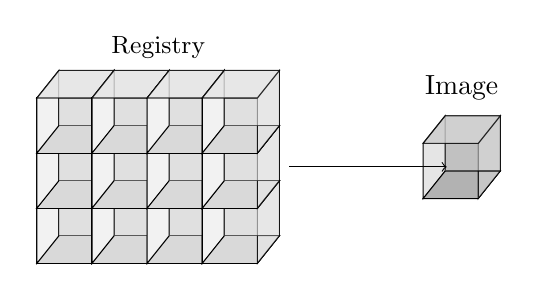
\begin{tikzpicture}

  \registry{R0}{0.7}{3}{4}{} %location  
  \cube{C1}{0.7}{black}{right = 0cm and 2cm of R0};
  \node[above = 0.25cm of C1_north] (IMAGE_LABEL) {Image};
  
  %\node[container, right = 0cm and 2cm of C1_east] (IMAGE) {};
  %\draw[->] (R0C13.east) -- (C1.west);
  \draw[->] (R0.east) -- (C1.west);
  %\draw[->] (C1_east) -- (C);
\end{tikzpicture}
\caption{Registries and Images}
\end{figure}

\subsection{API Server}

All components of an OpenShift cluster, internal and external, communicate through a Hypertext 
Transfer Protocol (\textbf{HTTP}) interface. Within every OpenShift cluster resides one application programming 
interface (\textbf{API}) server which interprets the HTTP commands and executes the respective 
operations server side. 

%Distributed openshift and pod diagram
%-----------------------------------------------%
% Core Components Diagram
%-----------------------------------------------%
\begin{figure}
\begin{tikzpicture}[node distance = 1cm and 0cm]
  % OpenShift layer
  \tikzstyle{OS_LAYER} = [app_stack, OS_COLOR, minimum width = 11cm, minimum height = 6.0cm]
  \tikzstyle{OS_CLIENT} = [app_stack, OS_COLOR, minimum width = 3cm, minimum height = 2.0cm]
  \tikzstyle{image} = [c_full, fill=white!20, opacity=0.5]
  \tikzstyle{mw} = [minimum width=15.0cm]
  \tikzstyle{mh} = [minimum height=7.5cm]
  \tikzstyle{link} = [-, thick, opacity=0.3]
  \xdef\pLabel{PRJ0}


  \node[USR_LAYER, mw, mh] (USR) {};
  \node[KRN_LAYER, mw, below = 0cm and 0cm of USR.south] (KRN) {Kernel};
  \node[HW_LAYER,  mw, minimum height = 2cm, below = 0cm and 0cm of KRN.north, anchor=north] (HW) {Hardware};

  \node[OS_LAYER, left = 0cm and -4cm of USR.center] (OS) {};
  \node[above= 0.1cm of OS.south] (OS_LABEL) {\color{white} OpenShift Server};
  
  \node [below = 0cm of  HW.south] (HM) {Physical Machine};
  \path[->, thin, to path={-| (\tikztotarget)}]
    (HM.west) edge (HW.south west)
    (HM.east) edge (HW.south east);

  \node[box, minimum height = 1.75cm, minimum width = 5.25cm, DK_COLOR, below left= 0.25cm and -1.25cm of OS.center,
       label={[label distance=-0.65cm]270:Container Engine}] (DK) {};
  \containers{0}{8}{8}{above left= 0.75cm and 2cm of DK.south};
  
  \project{\pLabel}{0.5}{8}{4}{above left = 1.50cm and 0.0cm of DK}
  \project{\pLabel}{0.5}{8}{4}{above left = 1.50cm and 0.0cm of DK}

  \node[right= 3.0cm of OS.center, label={[align=center]center:API\\Server}] (OAPI) {
    \begin{tikzpicture}
      \fill[thick, white, opacity=0.5] \gear{8}{1.0}{0.9}{10}{2}{0.3};
    \end{tikzpicture}};

  \node[right= 0cm and 1cm of \pLabel.east] () {};
  \node[OS_CLIENT, below right = 1.0cm and 4.25cm of USR.center, label={[align=center,]center:OpenShift\\\color{white}Client}] (OS_CLIENT) {};
  
  \tikzstyle{d_seg_color} = [fill=black!10]
  \tikzstyle{d_seg} = [cylinder, d_seg_color,draw, shape border rotate=90, thin, minimum width = 1.7cm, minimum height = 1.5cm]
  \node[d_seg, below= 3.90cm of OAPI.south] (D0) {};
  \node[below= 0cm of D0.center ] (D0_label) {Disk};

  %--------------------
  % API CONNECTIONS
  %--------------------
  \node[right = 0cm and 1cm of PRJ0.east] (API_NORTH_CONN) {};
  \path[link, line width=2.8pt, white, to path={|- (\tikztotarget)}]
    (OAPI.north) edge (API_NORTH_CONN.center)
    (API_NORTH_CONN.center) edge (PRJ0.east)
    (OAPI.east) edge (USR.east)
    (OAPI.south) edge (D0.north)
    (OS_CLIENT.north) edge (OAPI.340);

  \xdef\dis{0.05}
  \node[below = 2.00 cm of PRJ0P0C00] (CONN0_0) {};
  \node[below = 1.50 cm of PRJ0P0C01] (CONN1_0) {};
  \node[below = 1.25 cm of PRJ0P1C00] (CONN2_0) {};
  \node[below = 1.00 cm of PRJ0P1C01] (CONN3_0) {};
  \node[below = 1.50 cm of PRJ0P2C00] (CONN4_0) {};
  \node[below = 1.50 cm of PRJ0P2C01] (CONN5_0) {};
  \node[below = 1.50 cm of PRJ0P3C00] (CONN6_0) {};
  \node[below = 2.00 cm of PRJ0P3C01] (CONN7_0) {};

  \path[link, to path={|- (\tikztotarget)}]
    (CONN0_0.center) edge (C0_0.west)
    (C1_0.north) edge (CONN1_0.center)
    (C2_0.north) edge (CONN4_0.center)
    (C3_0.north) edge (CONN2_0.center)
    (C4_0.north) edge (CONN3_0.center)
    (C5_0.north) edge (CONN5_0.center)
    (C6_0.north) edge (CONN6_0.center)
    (CONN7_0.center) edge (C7_0.east);

  \path[link, ->]
    (CONN0_0.center) edge (PRJ0P0C00.south)
    (CONN1_0.center) edge (PRJ0P0C01.south)
    (CONN2_0.center) edge (PRJ0P1C00.south)
    (CONN3_0.center) edge (PRJ0P1C01.south)
    (CONN4_0.center) edge (PRJ0P2C00.south)
    (CONN5_0.center) edge (PRJ0P2C01.south)
    (CONN6_0.center) edge (PRJ0P3C00.south)
    (CONN7_0.center) edge (PRJ0P3C01.south);

  \node[right = 0.0cm and 3.00cm of PRJ0P3.10] (CONN0_P3) {};
  \node[right = 0.0cm and 2.75cm of PRJ0P3.350](CONN1_P3) {};

  \tikzstyle{port} = [rectangle, minimum height = 0.05cm, minimum width = 4cm, fill=white]
  \node[port, rotate=90, minimum width = 1cm, above= 0.0cm and 1cm of PRJ0P0.north, anchor=west] (PORT0) {\tiny 010101010};
  \node[port, rotate=90, minimum width = 1cm, above= 0.0cm and 1cm of PRJ0P1.north, anchor=west] (PORT1) {\tiny 010101010};
  %\node[port, rotate=90, minimum width = 1cm, above= 0.0cm and 1cm of PRJ0P2.north, anchor=west] (PORT2) {\tiny 010101010};
  %\node[port, rotate=90, minimum width = 1cm, above= 0.0cm and 1cm of PRJ0P3.north, anchor=west] (PORT3) {\tiny 010101010};

  \node[rotate=90, above right = -0.7cm and 0.0cm of PORT0] (PORT0_LABEL) {\scriptsize Port};
  \node[rotate=90, above right = -0.7cm and 0.0cm of PORT1] (PORT1_LABEL) {\scriptsize Port};
  %\node[rotate=90, above right = -0.7cm and 0.0cm of PORT2] (PORT1_LABEL) {\scriptsize Port};
  %\node[rotate=90, above right = -0.7cm and 0.0cm of PORT3] (PORT3_LABEL) {\scriptsize Port};

  %\user{user1}{}{above right = 1.65cm and 3.5 cmof OS.center}
  %\user{user2}{}{right= 0cm and 1cm of user1}
  %\user{user3}{}{right= 0cm and 1cm of user2}  

  %\tikzstyle{sa} = [fill=white, opacity=0.4, minimum width = 3.5cm];
  
  %\node[sa, fit=(user1_FIT)(user2_FIT)(user3_FIT), draw] (SA) {};
  %\node[above = 0cm of SA.north] (SA_LABEL) {Service Account};
  %\node[port, sa, left = 0cm and 0.0cm of SA.west] () {};
  
  %\node[below = 0.05cm of SA.south] (USER_LABEL) {User};
  %\path[link, ->] (USER_LABEL) edge (user2);
   
  %\node[rectangle, fill= white, above right= of OS] (SA) {};
  %\user{user1}{}{}

\end{tikzpicture}
\caption{API Server}
\end{figure}

This means that any programming language can manipulate an OpenShift cluster so long as that
language can send HTTP requests. However, OpenShift already provides client tools for 
common operations. In the following example, the client command, (\textbf{oc whoami -t}), is used to 
retrieve the authorization token to take a look at the HTTP interface, or Representational 
State Transfer (\textbf{REST}) API:    

\begin{lstlisting}[style=shell]
# After logging into a local openshift cluster ( oc login https:localhost:8443 )
curl -X GET -H "Authorization Bearer $(oc whoami -t)" https://localhost:8443/oapi/v1 --insecure
{
  "kind": "APIResourceList",
  "groupVersion": "v1",
  "resources": [
    {
      "name": "appliedclusterresourcequotas",
      "namespaced": true,
      "kind": "AppliedClusterResourceQuota",
      "verbs": [
        "get",
        "list"
      ]
    }, 
    {
      "name": "buildconfigs",
      "namespaced": true,
      "kind": "BuildConfig",
      "verbs": [
        "create",
        "delete",
        "deletecollection",
        "get",
        "list",
        "patch",
        "update",
        "watch"
      ]
    },
...
\end{lstlisting}

%\begin{enumerate}[(1)]
% \item service accounts
%\end{enumerate}
%In or
%A service account is like a low privledged user

%OpenShift keeps all of its recipes in a recipe cubby know as a registry. When a programmer wants a head start on their application,
%or write a new recipe, a image is chosen as the baseline

%- Add a section on the catalogue \n
%- Diff between OS image and docker image \n
%- How images are created \n
%- imagestreams \n
%- section on template \n
%- fix up cube code

%\section{TODO}
%\begin{enumerate}
%  \item Pods and Services
%  \item Builds and Image Streams
%  \item Container Registry
%  \item Web console
%  \item Builds and Image Streams
%  \item Deployments
%  \item Templates
%\end{enumerate}

\iffalse
\begin{figure}
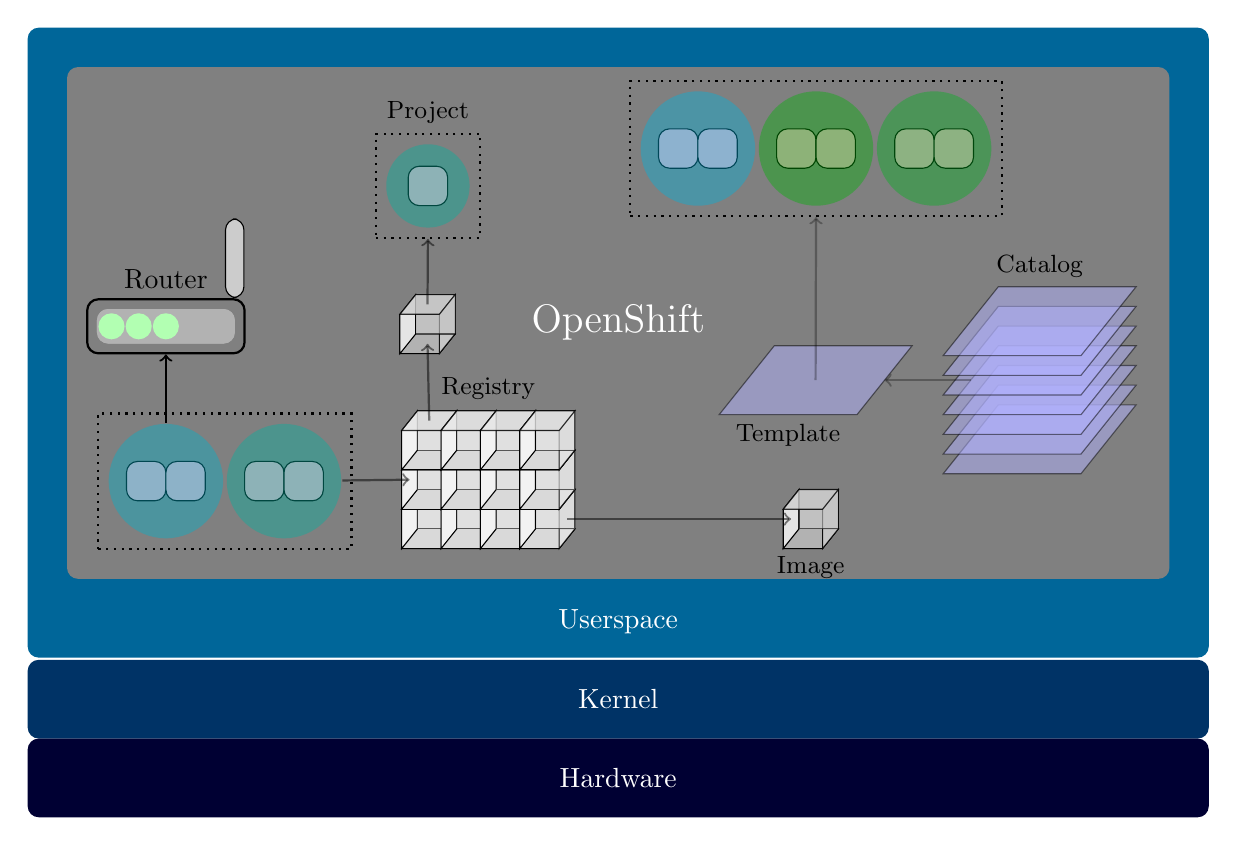
\begin{tikzpicture}[node distance = 1cm and 0cm]
  % OpenShift layer
  \tikzstyle{OS_LAYER} = [app_stack, OS_COLOR, minimum width = 14cm, minimum height = 6.5cm]
  \tikzstyle{image} = [c_full, fill=white!20, opacity=0.5]
  \tikzstyle{mw} = [minimum width=15.0cm]
  \tikzstyle{mh} = [minimum height=8.0cm]

  \node[USR_LAYER, mw, mh] (USR) {};
  \node[KRN_LAYER, mw, below = 0cm and 0cm of USR.south] (KRN) {Kernel};
  \node[HW_LAYER,  mw, below = 0cm and 0cm of KRN.north, anchor=north] (HW) {Hardware};

  %\node[HM_LAYER, mw] (HM_1) {Host Machine 1};
  %\node[HM_LAYER, mw, right=of HM_1] (HM_2) {Host Machine 2};
  %\node[HM_LAYER, mw, right=of HM_2] (HM_3) {Host Machine 3};
  \node[OS_LAYER, above=1cm of USR.south] (OS) {\Large \color{white} OpenShift};
  %\node[HM_LAYER, mw] (MB_1) {Host Machine 1};

  \project{PRJ0}{0.5}{4}{2}{above left = 0.75cm and 6.5cm of OS.south}

  %        id size rows cols location
  \registry{R0}{0.5}{3}{4}{above left= 0.35cm and 2.5cm of OS.south} %location  
  \path[->, opacity=0.5, thick] (PRJ0P1) edge (R0C10_west);

  \router{ROUTE0}{1.75}{above= 1.0cm of PRJ0P0}
  \path[->, thick] (PRJ0P0) edge (ROUTE0);

  \cube{C1}{0.5}{black}{above= 1cm and 0.0 cm of R0C20_north }; % location
  \path[->, thick, opacity=0.5] (R0C20_north) edge (C1_south);

  \project{PRJ1}{0.5}{1}{1}{above left = 1cm and 0.5cm of  C1_north}
  \node[above= 0cm of PRJ1.north] (PRJ1_label) {\small Project};
  \path[->, thick, opacity=0.5] (C1_north) edge (PRJ1.south);

  %     id size color    location
  \cube{C0}{0.5}{black}{right= 0cm and 3.5 cm of R0C02 }; % location
  \node[below= 0.10cm of C0_south] (C0_label) {\small Image};
  \path[->, thick, opacity=0.5] (R0C03_east) edge (C0_west);
  
  \catalog{CAT0}{1.75}{7}{above right = 1.75cm and 5.0cm of OS.south};
  \template{T0}{1.75}{blue}{left = 2.5cm of CAT0T3};
  \node[below= 0cm of T0_south] (T0_label) {\small Template};
  \path[->, thick, opacity=0.3] (CAT0T3_west) edge (T0_east);

  \project{PRJ2}{0.5}{6}{3}{above left= 2cm and 2.60cm of  T0_north}
  \path[->, thick, opacity=0.3] (T0_center) edge (PRJ2.south);

 % \path[->, thick, opacity=0.3] (CO_north) edge (T0_label);

\end{tikzpicture}
\end{figure}
\fi

%
%
%\section{Build}
%A build is an method of creating container images that can run on OpenShift

%- Need visual of an image
%- Need visual for build

%BuildConfig ---> Like Blueprint schematic
%
%\begin{figure}
%\begin{tikzpicture}[node distance = 1cm and 0cm]
%   \node[circle, fill=blue] (ph) {PlaceHolder};
%
%\end{tikzpicture}
%\caption{Build Config}
%\end{figure}

%\section{Container Registry}
%OpenShift is able to store the blueprints for applications in what is know as a registry

%\section{Image Stream}
%"Comprises of any number of container images identified by tages / Virtual view of related images"
%A collection of image references, a way to mass import container images into OpenShift
%Keeps track of images within registry

%importing a tag or image into an image stream?

---------------------------------------------------------------------------------------------------- \\
 WIP \\
---------------------------------------------------------------------------------------------------- \\
\end{document}

